\documentclass[12pt]{article}
\usepackage[usenames,dvipsnames]{color}
\usepackage{listings}
\usepackage{graphicx}
\usepackage{fancyhdr}
\usepackage{framed}
\usepackage[T1]{fontenc}
\usepackage[toc,page]{appendix}
\usepackage[utf8]{inputenc}
\usepackage[brazil]{babel}
\usepackage{fancyvrb}
\usepackage[hmargin=2cm,vmargin=2cm]{geometry}
\usepackage{lastpage}
\usepackage{pdfpages}
\usepackage{makeidx}
\usepackage{hyperref}
\pagestyle{fancy}
\usepackage{enumitem}
% cabecalho e rodapé
\setlength{\headheight}{120pt}
\setlength{\textheight}{550pt}
\renewcommand{\headrulewidth}{0pt}
\lhead{
\includegraphics[scale=0.03]{brasao.png}}
\rhead{
\includegraphics[scale=0.4]{logo-pnud.png}}
\cfoot{\textbf{\ProjectCode\ - Inovando a democracia participativa}}
\rfoot{\thepage}

\hyphenation{par-ti-ci-pa-ção}
\bibliographystyle{ieeetr}

% definições sobre o autor e o produto
\newcommand{\MyName}{Renato Fabbri}
\newcommand{\MySurnameForename}{Fabbri, Renato}
\newcommand{\SupervisorName}{Gabriella Vieira Oliveira Gonçalves}
\newcommand{\MyEmail}{renato.fabbri@gmail.com}
\newcommand{\ContractNumber}{2013/000566}
\newcommand{\ContractYear}{2014}
\newcommand{\ProjectCode}{Projeto BRA/12/018}
\newcommand{\NomeSecretaria}{Secretaria Geral da Presidência da República}
\newcommand{\SiglaSecretaria}{SG/PR}
\newcommand{\ProductNumber}{03}
\newcommand{\ProductTitle}{Ferramentas assistidas de categorização de conteúdo}
\newcommand{\ProductSubtitle}{Com Processamento de Linguagem Natural e de Redes Complexas, adaptadas para o ambiente do portal federal de participação social (Participa.br)}
\newcommand{\ProductDescription}{"Ferramentas assistidas de categorização de conteúdo: Com Processamento de Linguagem Natural e de Redes Complexas, adaptadas para o ambiente do portal de participação."
}

\newcommand{\ProductValue}{R\$ 10,800 (dez mil e oitocentos reais)}
\newcommand{\ObjetoContratacao}{
Aporte de conhecimentos e tecnologias para especificação de vocabulário e ferramentas assistidas que utilizam processamento de linguagem natural e análise de redes complexas para o conteúdo do portal da participação social.
}
\newcommand{\DataEntrega}{27 Julho de 2014}
\newcommand{\PalavrasChave}{reconhecimento de padrões, redes complexas, processamento de linguagem natural, participação social}

% lista de abreviações
\makeindex

\begin{document}

\newgeometry{hmargin=3cm,vmargin=1.5cm}
\begin{center}
\thispagestyle{empty}
{\color{MidnightBlue}


\includegraphics[scale=0.9]{logo-pnud.png}

\vspace{4cm}

{\bf \large \ProjectCode\ - Desenvolvimento de Metodologias
de Articulação e Gestão de Políticas Públicas para Promoção da Democracia
Participativa}

\vspace{1.5cm}

{\bf \large Produto \ProductNumber\ -\ \ProductTitle}

\vspace{1.5cm}

\ProductSubtitle

\vspace{4cm}

\MyName

\vspace{2cm}

}


\includegraphics[scale=0.04]{brasao.png} \\
{\bf \small \NomeSecretaria}

\end{center}
\restoregeometry
\newpage

\newgeometry{hmargin=3cm,vmargin=1.5cm}
\addtolength{\topmargin}{2.5cm}
\thispagestyle{empty}
{\color{MidnightBlue}

{\bf \LARGE Produto \ProductNumber\ -\ \ProductTitle}

\hrulefill

\vspace{1cm}

\begin{center}

{\bf \large Contrato n. \ContractNumber}

\vspace{1.5cm}

{\bf \large Objeto da contratação: \ObjetoContratacao}

\end{center}

\vspace{3.2cm}

Valor do produto: \ProductValue

\vspace{1.2cm}

Data de entrega: \DataEntrega

\vspace{1.2cm}

Nome do consultor: \MyName

\vspace{1.2cm}

Nome da supervisora: \SupervisorName

}

\vspace{2cm}

\begin{center}

\includegraphics[scale=0.04]{brasao.png} \\
{\bf \small \NomeSecretaria}
\end{center}

\restoregeometry
\newpage

\newgeometry{hmargin=3cm,vmargin=1.5cm}
\addtolength{\topmargin}{5cm}
\thispagestyle{empty}

\begin{framed}

{\raggedright \MySurnameForename} \\

\ProductTitle: \ProductSubtitle\ / \ContractYear. \\

Total de folhas: \pageref{LastPage} \\

\vspace{1cm}

Supervisor: \SupervisorName \\

\SiglaSecretaria \\

\NomeSecretaria \\

Palavras-chave: \PalavrasChave. \\

\end{framed}

\vspace{3cm}

{\raggedright 
\includegraphics{licenca-cc-by-nc.png} \ Esta obra é licenciada sob
uma licença Creative Commons - Atribuição-NãoComercial. 4.0 Internacional.}

\restoregeometry
\newpage

\tableofcontents
\newpage


\begin{abstract}
Este documento descreve procedimentos selecionados para categorização de conteúdo do portal federal de participação social (Participa.br). O produto relacionado no termo de referência desta consultoria preve somente propostas de especificações e códigos. Dado o aspecto prático do trabalho, estão descritas implementações e códigos operantes multiplataforma (linux/mac/windows). Parte deste trabalho é acessível online via http, como os scripts no IPython Notebook e o endpoint SparQL que serve os dados do Participa.br por critérios semânticos.\\

{\bf Palavras-chave:} \PalavrasChave.
\end{abstract}
\newpage

\section{Introdução}
\subsection{Contexto e importância da consultoria}
Em confluência com o portal federal de participação social (Participa.br), e o Plano Nacinal de Participação Social (PNPS), esta consultoria propõe métodos de classificação e priorização de conteúdo e formas de autorregulação para o portal. O presente produto apresenta uma seleção de métodos para classificação de conteúdo. Dadas a pertinência para o contexto participativo e a simplicidade, são apresentadas a classificação via 1) conectividade dos autores e 2) características dos documentos.
\subsection{Contexto e importância do Produto}
\begin{itemize}
    \item Este Produto, através da classificação de conteúdos, visa 1) explicitar propriedades do sistema considerado; 2) permitir observação de conteúdos produzidos por nichos ou características em comum; 3) facilitar a assimilação das informações produzidas pelos participantes.
    \item Estão planejadas a incorporação destes métodos no funcionamento do Participa.br.
    \item Os participantes, através da vivência em suas redes, tendem a apropriar-se delas e buscar processamentos para categorizar os conteúdos e os resumir, como ocorreu com os dashboards de IRC, como acontece com os apps do Facebook e os artigos sobre o Twitter.
    \item A especialização conectiva dos agentes sociais, e do texto produzido por indivíduos e grupos, é um fenômeno reconhecido. Há aproveitamento destas diferenciações pela conectividade. A entrega deste ferramental ao poder federal e à sociedade, via iniciativa conjunta (Participa.br), capacita a democracia participativa.
\begin{itemize}
        \item Permite análise dos dados dos processos, fortalecendo a transparência e dificultando falcatruas.
        \item Permite a escolha, via critérios públicos, de articuladores de processos participativos.
        \item Permite a remuneração de horas de dedicação de participantes escolhidos.
        \item Permite aproveitamento aberto e conjunto de previsões estatísticas e leis naturais.
        \item Permite o estabelecimento de dinâmicas (trilhas participativas) para elaboração conjunta
de documentos que aproveitam as propriedades naturais destes sistemas.
\end{itemize}
\end{itemize}


\section{Desenvolvimento}
\subsection{Etapas de desenvolvimento}
\subsubsection{Estudo ontológico e triplificação dos dados para API de acesso}
Para viabilizar a classificação de conteúdos do portal participativo, em confluência com as propostas de web semântica desta consultoria e do Participa.br, foi necessário uma abordagem ontológica dos aspectos envolvidos no Participa.br, assim como a triplificação dos dados. Para isso, a OPS (Ontologia de Participação Social) foi revisada, com melhoras substanciais, também a OPA (Ontologia do Participa.br) foi criada~\cite{OPS,OPA}. Já a representação dos dados do Participa.br em triplas RDF envolveu o uso destas e diversas outras ontologias~\cite{triplifica}.
\subsubsection{Instanciação de um Fuseki/Jena e um IPython Notebook}

Os dados triplificados podem ser usados diretamente em algum aplicativo ou programa. A forma padrão de disponibilizar dados em RDF, porém, é através de um endpoint, que prepara os dados na RAM para buscas especificadas via SparQL. Está online um endpoint Jena para consultas SparQL via HTTP. Também uma seleção dos scripts em Python estão disponíveis através de navegadores comuns, como o Firefox ou o Chrom(e,um). {\bf Veja os Anexos~\ref{subsec:etp}-\ref{subsec:online}}.
\subsubsection{Classificação dos textos (mineração de texto / processamento de linguagem natural)}
As possibilidades de classificação de conteúdo com base nos textos são inúmeras. Nesta subsubseção, são apontados alguns dos caminhos considerados.
\begin{itemize}
    \item Através de uso de textos previamente classificados, pode-se treinar classificadores automatizados. Este é o chamado “aprendizado supervisionado” de máquina. As técnicas atualmente em uso são inúmeras (redes neurais, algorítmos genéticos, etc). Para  exemplificação, foi implementado uma aprendizagem Bayesiana. É o tipo de classificação normalmente usada para lidar com etiquetação de mensagens e com personas. No Anexo~\ref{subsec:etp} consta uma implementação.
    \item A classificação de objetos sem classes previamente definidas, com base somente nas propriedades dos objetos, é conhecido como ``aprendizado não supervisionado''. Pode-se impor a existencia de 2 classes (com base no balanço estrutural~\cite{easley}), ou mais classes, de forma a maximizar a dispersão inter-classe e diminuir a dispersão intra-classe. Este processo pode ser útil para observar nichos nas atividades, mesmo sem um conjunto de mensagens classificadas de antemão.
    \item Classificação de mensagens similares às escolhidas. Esta distância pode ser euclidiana no espaço de contagem de palavras, ou calculada via redes semânticas (e.g. wordnet).
    \item Classificação via contexto similar da palavra ou via simples incidência da palavra. Assemelha-se aos buscadores usuais, com capacidades para lidar com contexto (outras palavras, tipo de autor, classificação da mensagem).
    \item Ranqueamentos para mensagens, autores e palavras:

\begin{itemize}
        \item Mais adjetivos, mais substantivos, mais pontuações, etc. 
        \item Maior tamanho médio das palavras ou variedade de tamahos (desvio padrão). O Anexo~\ref{subsec:srl} apresenta uma implementação.
        \item Frases mais longas em caracteres ou em palavras, variedade de tamanhos (desvio padrão).
        \item Uso de limiares para o rankeamento, p.ex.: os participantes que mais usam adjetivos (ou escrevem mensagens de mobilização) dentre os que possuem mais de 10 mensagens. O Anexo~\ref{subsec:srl} apresenta uma implementação.
\end{itemize}
\end{itemize}
\subsubsection{Classificação dos agentes pela conectividade (Redes Complexas)}
\begin{itemize}
    \item Em geral, as redes formadas com os rastros de atividade digital são: redes de interação ou redes de relações. No participa, há, em especial, a rede de amizades entre os usuários (relações) e as redes de interação: quem responde quem, etc. O Anexo~\ref{subsec:intAm} exibe a formação destas redes.
    \item Pode-se classificar os usuários por comunidades detectadas nas redes. Veja o Anexo~\ref{subsec:com}.
    \item Ranqueamento por centralidade é um dos recursos mais comuns. Há medidas de centralidade com base da conectividade (grau), intermediação (betweeness) proximidade (closeness) e ainda outras medidas. O Anexo~\ref{subsec:rkRd} exibe rankeamento dos participantes por estas medidas.
    \item As redes sociais, por serem em geral “livres de escala”, possuem especialização dos agentes, canonicamente pensados em “hubs”, “intermediários” e “periféricos”. Estes setores podem ser obtidos com mais propriedade comparando o histograma de conectividade da rede real com uma Erdös-Renyi com o mesmo número de vértices e arestas. Veja o Anexos~\ref{subsec:setCon} para uma implementação em Python para obtenção dos integrantes destes setores com base nos dados do Participa.br.
\end{itemize}
\subsubsection{Combinação de medidas de RC, PLN e outras}
\begin{itemize}
    \item As medidas de redes e de texto podem ser combinadas para melhorar a qualidade dos classificadores de mensagem. As estabilidades nestas medidas sugerem que hajam outliers e uma tipologia pertinente para os agentes~\cite{fabbri1, fabbri2}.
    \item Medidas de uso do sítio e do perfil do participante podem enriquecer os classificadores.
    \item Um exemplo de classificação de conteúdo, com base na classificação conectiva do autor, está no Anexo~\ref{subsec:misto}.
\end{itemize}
\subsubsection{Aquisição de dados classificados}
Para o aprendizado supervisionado (etiquetação automática, análise de sentimento, etc), é utilizado um conjunto de dados etiquetados de antemão, para “treinar” o classificador.
Nas áreas de comunicação e monitoramento, são etiquetadas à mão as mensagens como positivas, negativas e neutras e em outras classes de interesse (e.g. geolocalizações, assuntos). Os autores são classificados em personas (autor masculino, feminino, ativista, militante, curioso, etc). Esta classificação manual pode servir para treinar um classificador público, talvez do Participa.br mesmo, especialmente se revisada por uma ou mais pessoas.
\subsection{Justificativa do método}
\begin{itemize}
    \item Classificações mais fundamentais: os métodos utilizados (bag-of-words, aprendizado bayesiano, medidas de grau e betweenness) são as mais usuais, além de facilitar a comparação e estabelecimento de benchmarks, possuem eficiência conhecida e significados mais facilmente compartilhados.
    \item Amadurecimento com equipe do Participa.br: há outros consultores e integrantes da SG/PR, e da sociedade civil, que compõem ou se comunicam com a equipe do Participa.br. Neste contexto, foram propostas e amadurecidas diversas possibilidades de classificação de conteúdos. Neste processo, foi decantado esta seleção, apresentada neste Produto.
\end{itemize}
\subsection{Justificativa das fontes}
\begin{itemize}
    \item Pesquisa científica: o autor é pesquisador nas áreas relacionadas com produção bibliográfica em revistas internacionais e em circulação nacional.
    \item Os frameworks computacionais utilizados (nltk, networkx, rdflib, jena, etc) são amadurecidos no mundo todo, em desenvolvimento aberto, com comunidades dedicadas e pública discussão.
    \item A equipe do Participa.br é uma equipe da SG/PR voltada para a participação social. Desta equipe provém boa parte dos avanços na participação social.
\end{itemize}
\subsection{Confronto entre os resultados esperados e os alcançados}
Este Produto preve “propostas de especificações e códigos” de classificação de conteúdo do Participa.br. Este Produto compreende estas propostas. Há, além disso, alguns resultados alcançados a mais:
\begin{itemize}
    \item Propostas operantes em códigos online, já integrado aos dados semânticos e disponibilização via endpoint SparQL. Veja IPython e Jena no Anexo~\ref{subsec:online}.
    \item Interfaces/frontends já estudadas para gráficos, reatividade e streaming (meteor+d3). Veja MMISSA, MM, Telões e MyNSA no Anexo~\ref{subsec:online}.
    \item Entrega, através dos resultados dos scripts, de uma breve análise do Participa.br em termos dos rastros digitais, dos conteúdos e dos usuários. Veja Anexos~\ref{subsec:etp}-\ref{subsec:csparql}.
\end{itemize}

Este documento e os scripts foram reunidos em um repositório git público usual~\cite{repoProd3}.

\section{Usos dos resultados}
O próximo Produto desta mesma consultoria possui foco na utilização destas classificações. Exemplos de usos estão topificados abaixo.
\begin{itemize}
    \item Navegação dos conteúdos do portal: facilitar a aquisição das informações de interesse; permite observar o conteúdo com base em características dos participantes (e.g. hub, periférico, intermediarios) ou dos conteúdos (e.g. fração de adjetivos ou classificada com rótulos X ou Y).
    \item Enriquecimento do legado semântico do Participa.br e outros portais: boa parte dos cálculos, necessário para obtenção das estatísticas e classificações, requerem recursos computacionais poderosos e técnicas nada triviais. Assim, os resultados podem ser disponibilizados junto aos dados, em RDF.
    \item Atribuição de função: através das estatísticas dos grupos, pode-se recompensar atores  ou convidá-los para atividades ou funções especiais.
    \item Resumos: usualmente dashboards, redes ou relações de palavras, visões gerais da entidade de interesse. A entidade pode ser um portal, uma comunidade, um usuário, uma trilha ou uma etapa participativa. Estes resumos são bastante úteis para valorizar as instâncias e orientar os participantes.
    \item Coleta destas informações para usos/ações: difusão de mídia, consultas, propostas, estudos, deliberações, etc.
\end{itemize}

\section{Conclusão}
A categorização de conteúdo do Participa.br pode ser feita de forma distribuída. Os dados, servidos por um endpoint SparQL, podem ser analisados por frontends, como um IPython Notebook, um ScrapperWiki ou um Meteor+d3 para visualizações interativas. Foi testado um intermediário em Flask para servir os dados já formatados para o frontend. Funcionou com serviços gratuitos do Heroku, Meteor e Mongo Labs, embora com limitações e alguns impasses para desenvolvimento em nuvem. Os Anexos~\ref{subsec:etp}-\ref{subsec:online} ao final deste documento, e o repositório git~\cite{repoProd3} são os resumos principais do Produto.
\subsection{Comentários, sugestões, recomendações}
\begin{itemize}
    \item Para boas aplicações de classificadores de conteúdo, é necessário uma quantidade grande de conteúdo classificado previamente, geralmente à mão. Assim, é pertinente a etiqeutação das mensagens com os parceiros da comunicação, para liberação junto aos dados semânticos e treino de classificadores.
    \item Como pode-se notar no Anexo~\ref{subsec:srl}, há bastante mensagem repetida. Embora este problema tenha sido tratado na utilização dos dados, é recomendado que seja corrigido o problema nos dados do Participa.br. Uma boa solução, embora não ideal, é a correção destes dados na triplificação deles.
\end{itemize}
\subsection{Impacto do Produto para a elaboração, gestão e/ou avaliação de políticas públicas de participação social}
\begin{itemize}
    \item Este produto facilita a apropriação dos processos participativos através da categorização de conteúdos e observação de suas características. 
    \item Este produto explicita a entrega das informações para a população, para observação distribuída.
    \item Este produto entrega, em tecnologias livres, ferramental de redes sociais, redes complexas e processamento de linguagem natural.
    \item Este produto entrega estes algoritmos em forma executável em navegadores HTTP comuns, como Firefox ou Chrome(um).
    \item Este produto entrega uma instância operante de acesso aos dados do Participa.br, em formato RDF e enriquecidos.
    \item Este produto faz uso efetivo de tecnologias de dados linkados / web semântica.
\end{itemize}
\subsection{Como o Produto deverá impactar o público-alvo das políticas públicas a que se refere}
\begin{itemize}
    \item Permitindo navegação seletiva pelos conteúdos disponíveis.
    \item Valorizando as instâncias e as tornando mais informativas, com resumos estatísticos e visuais.
    \item Explicitando propriedades dos processos participativos e usos destas propriedades.
    \item Integrando o portal federal de participação social (Participa.br) ao legado humano de dados linkados (via critérios semânticos).
    \item Permitindo critérios funcionais para atribuição de papéis para participantes. Por exemplo, a construção de um manifesto ou resumo final pode ser feito requisitando: de periféricos, os substantivos; de hubs, os adjetivos; e de intermediários, que formem o texto com aquelas palavras. Outra possibilidade é a remuneração de hubs pela participação efetuada ou a convocação de periféricos para oxigenar o processo participativo.
    \item Aproximando perfis técnicos pela qualidade das tecnologias utilizadas, pela da relevância dos dados sobre participação social e pela pertinência dos métodos.
\end{itemize}


\newpage
\bibliography{bibliografia}
\newpage
%\listoffigures
\section*{Abreviações e jargão}

OPS: Ontologia de participação Social

OPA: Ontologia do Participa.br

MMISSA: Monitoramento Massivo e Interativo da Sociedade pela Sociedade para Aproveitamento

AARS: A Análise de Redes Sociais

PNPS: Plano Nacional de Participação Social

RDF: Resource Description Framework

HTTP: Hypertext Transfer Protocol

SPARQL:  Simple Protocol and RDF Query Language

endpoint SPARQL: ponto de acesso, geralmente HTTP, a dados em RDF via buscas em SPARQL.

Participa.br: Portal federal de participação social.

IPython Notebook: instância online para rodar scritps Python

Mateor: arcabouço para páginas reativas e com funcionamento distribuído.

D3js: biblioteca de visualização de dados.

\newpage
\printindex
\newpage
%\section*{Anexos}
\begin{enumerate}
\item Classificação de conteúdo via mensagens etiquetadas e personas.
\item Seleção por rankeamento (tamanho de palavra) e limiar (número mínimo de palavras)
%\item Seleção por rankeamento de atividade dos usuários
\item Redes de amizade e de conteúdo do Participa.br
\begin{enumerate}
    \item Ordenação (ranking) por centralidade
    \item Setores conectivos
    \item Deteção de comunidades
\end{enumerate}
\item Exemplo em código computacional de classificação de conteúdo via conectividade dos participantes.
\item Script para testar o tempo de resposta do endpoint SparQL como conexão local e remota. OK
\item Experimentos online.
\end{enumerate}

\appendix
\section*{Anexos}
\addcontentsline{toc}{section}{Anexos}  
A seguir estão trechos de código Python que executam funções básicas de classificação de conteúdo do Participa.br ou úteis para isso.
Estes códigos estão executáveis online, acessíceis nos browsers web usuais (firefox, chrome(um)), através de um IPython Notebook. Mais informações no Anexo~\ref{subsec:online}.
%\appendixpage
%\section*{Anexos}
%\addcontentsline{toc}{section}{Anexos}  
\newcommand\invisiblesection[1]{%
  \refstepcounter{section}%
  \addcontentsline{toc}{section}{\protect\numberline{\thesection}#1}%
  \sectionmark{#1}}
\newcommand\invisiblesubsection[1]{%
  \refstepcounter{subsection}%
  \addcontentsline{toc}{subsection}{\protect\numberline{\thesubsection}#1}%
  \subsectionmark{#1}}

%\input{appendix.tex}


\invisiblesection{Classificação via etiquetas e personas}
\label{subsec:etp}
%\section*{1-Classificação via etiquetas e personas}
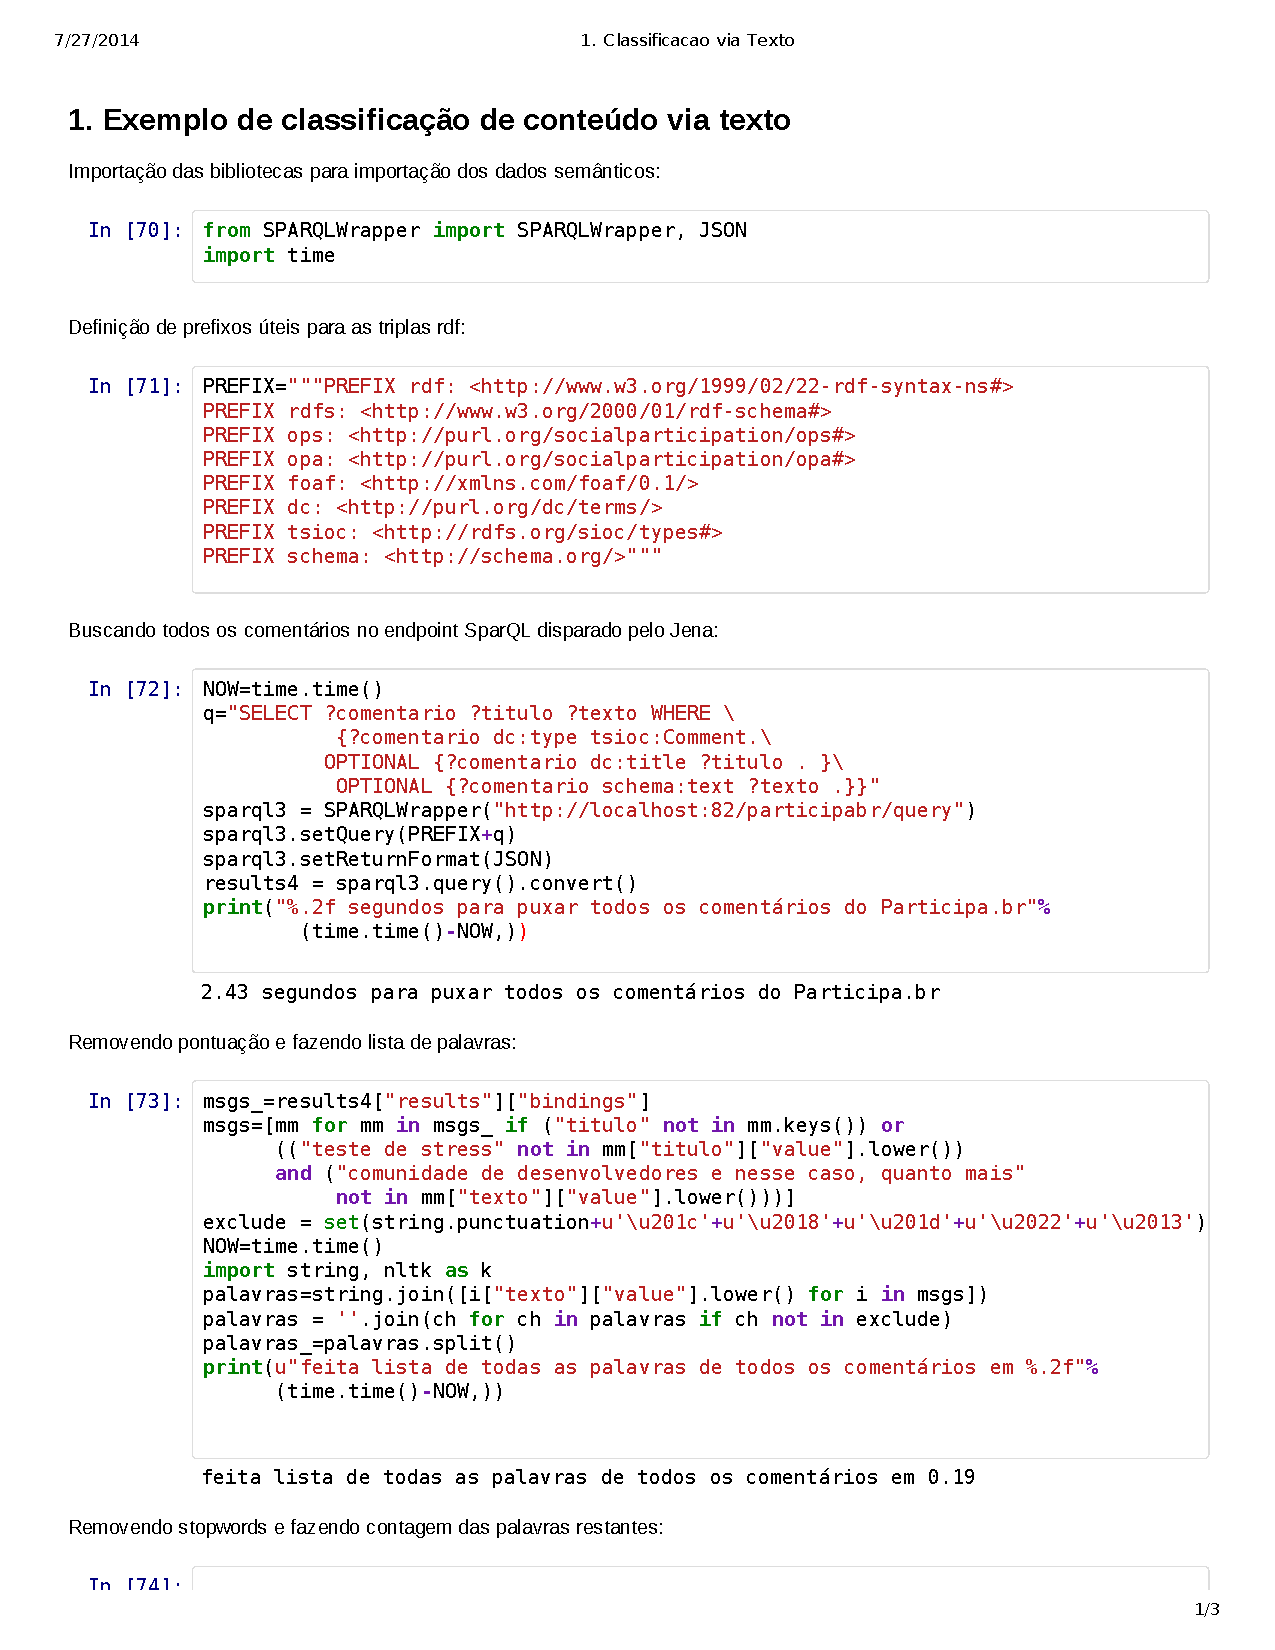
\includepdf[pages=-]{1-ExemploDeClassificacaoTexto.pdf}
\invisiblesection{Seleção por ranqueamento e limiar}
\label{subsec:srl}
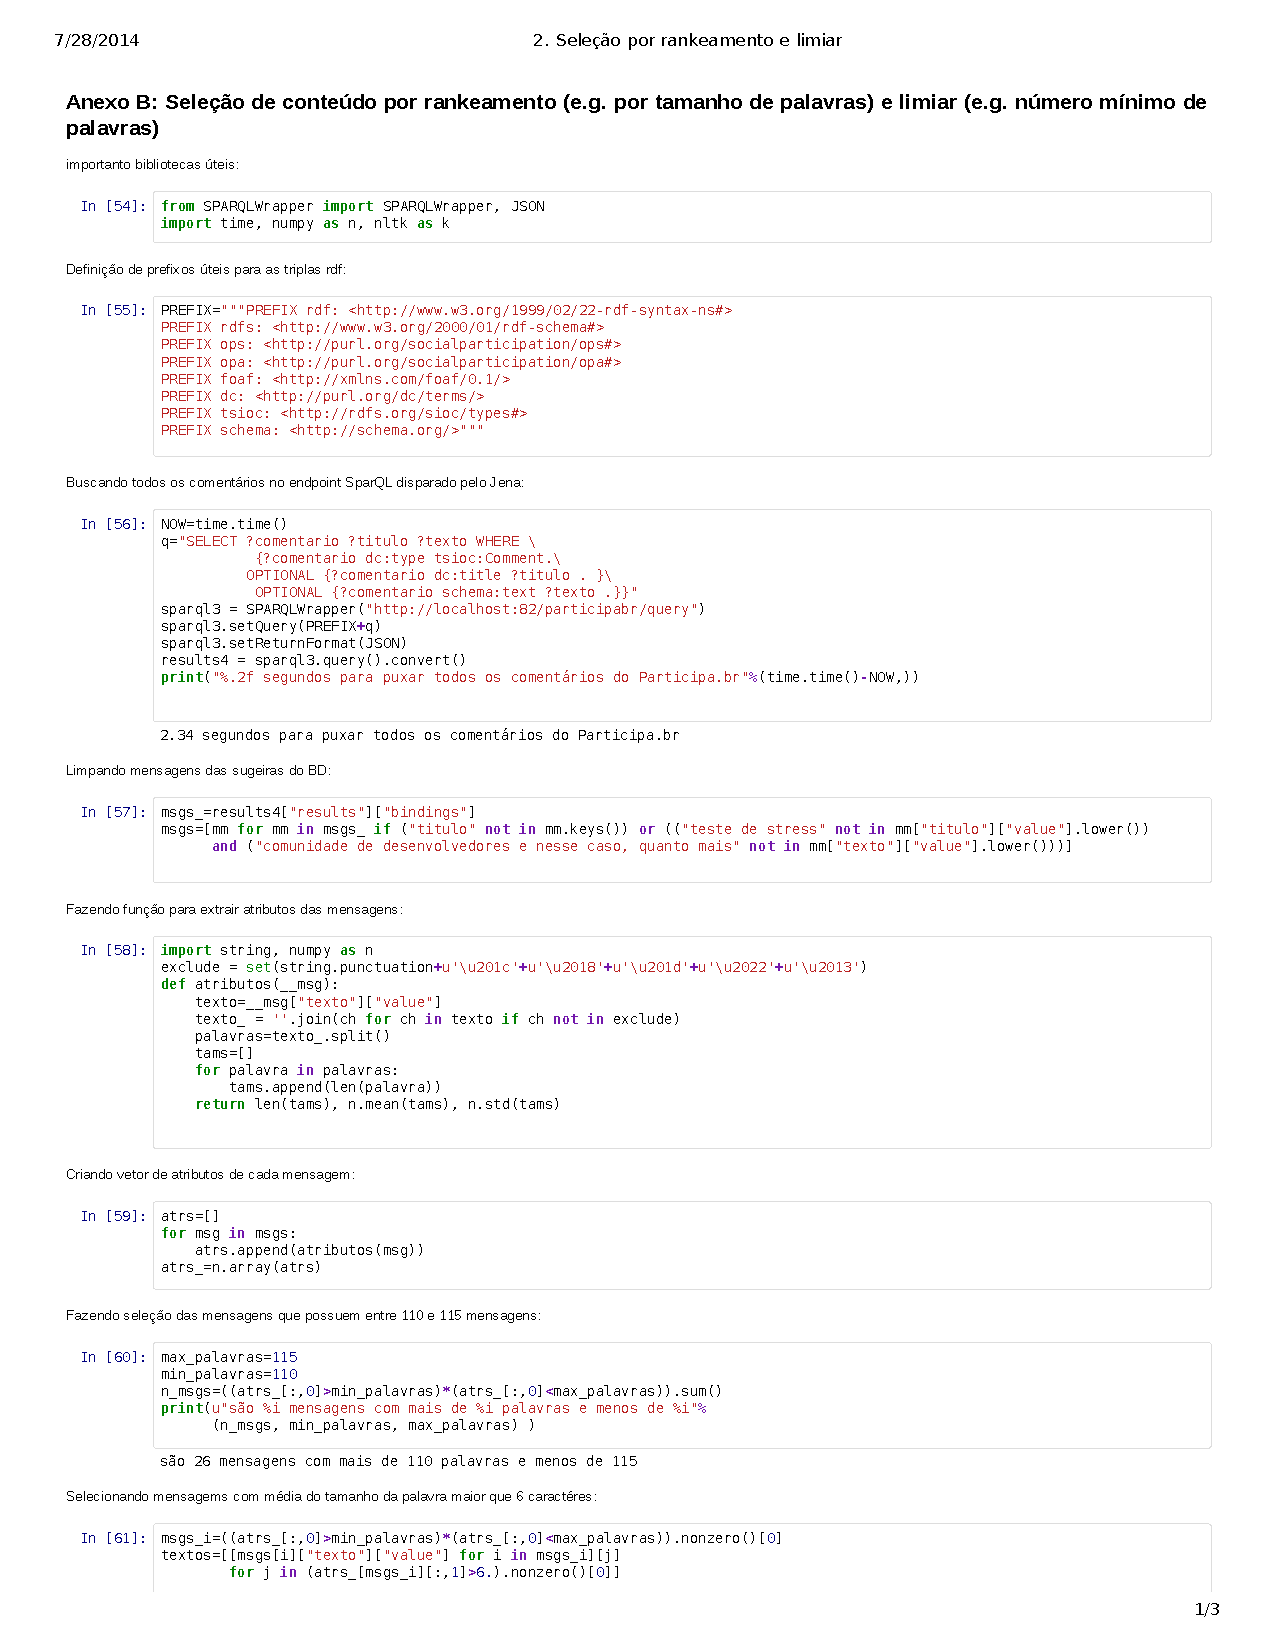
\includepdf[pages=-]{2-SelecaoRanqueamento.pdf}
\invisiblesection{Redes de interação e de amizade}\label{subsec:intAm}
\invisiblesubsection{Ordenação (ranking) por centralidade}\label{subsec:rkRd}
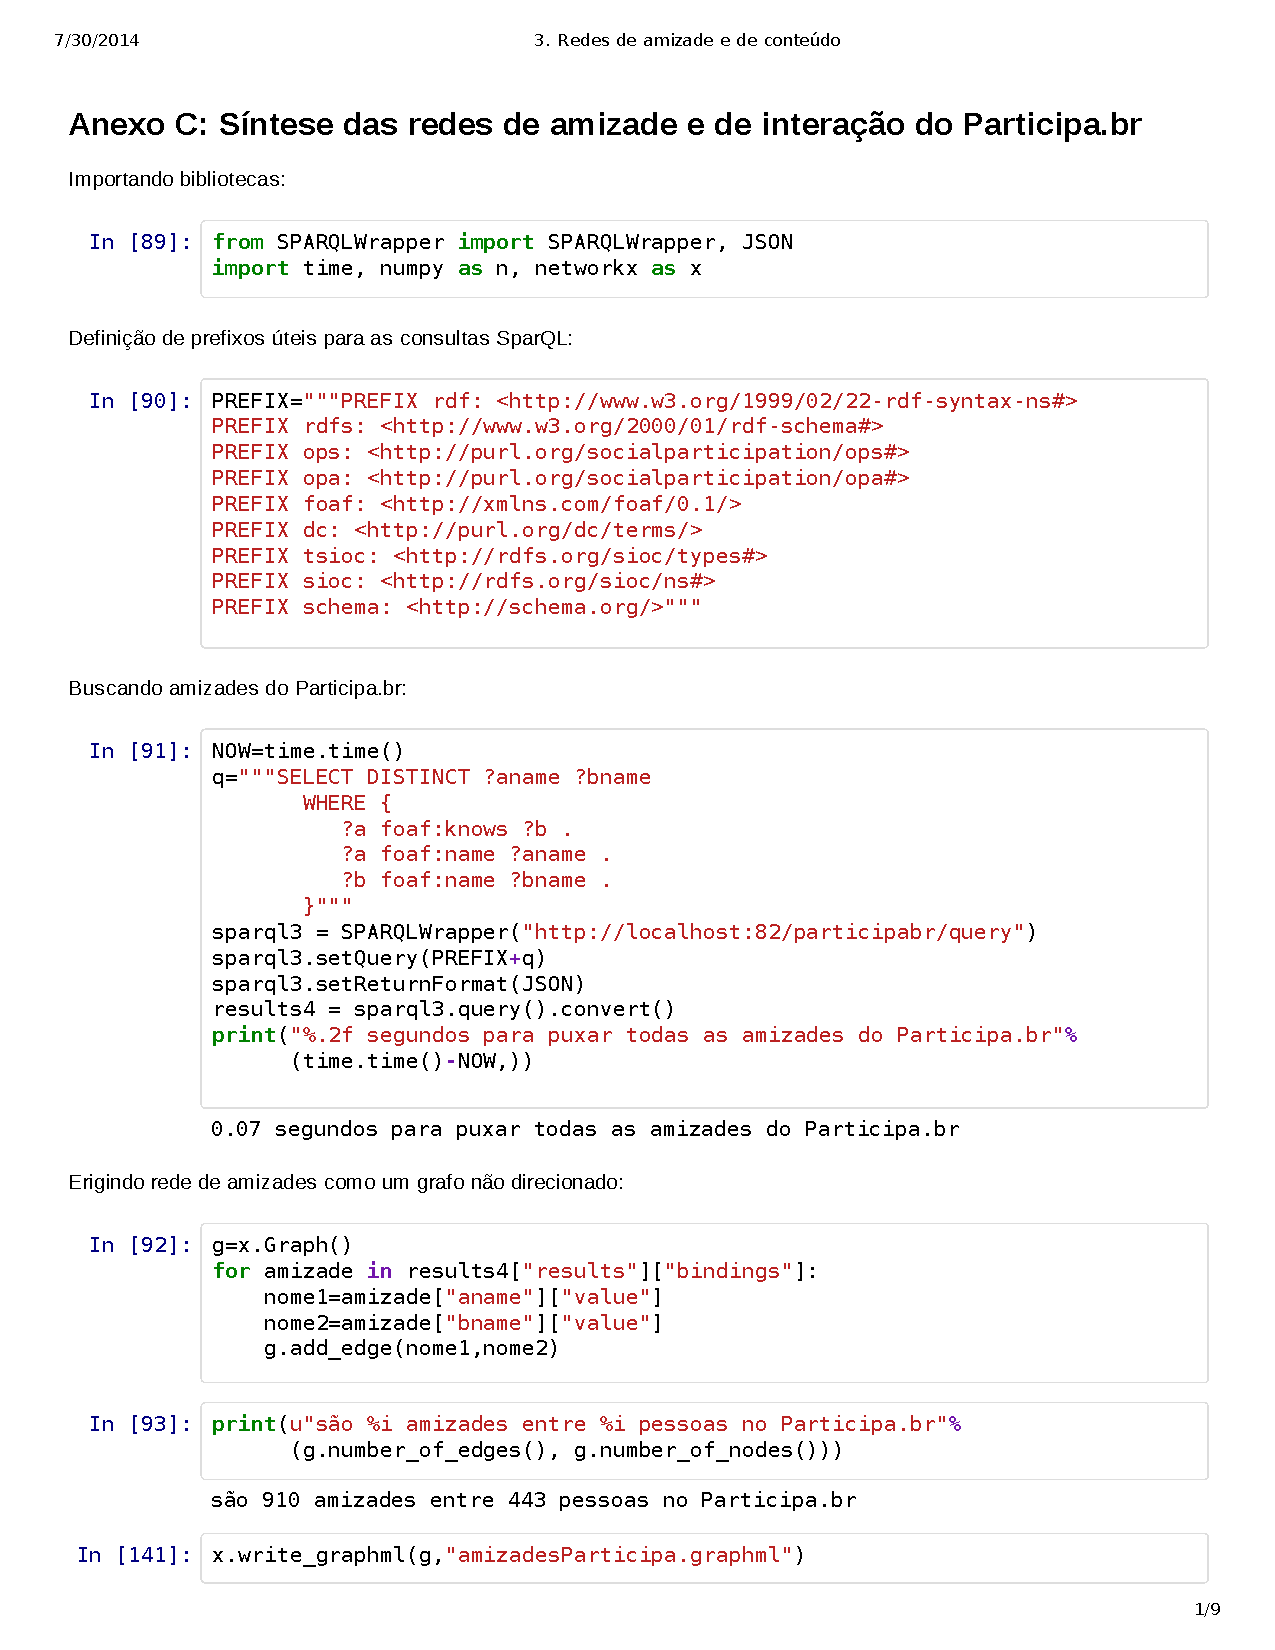
\includepdf[pages=-]{3-RedesAmizadeInteracao.pdf}
\invisiblesubsection{Setores conectivos}\label{subsec:setCon}
\invisiblesubsection{Detecção de comunidades}\label{subsec:com}
\invisiblesection{Classificação de conteúdo via conectividade dos participantes}\label{subsec:misto}
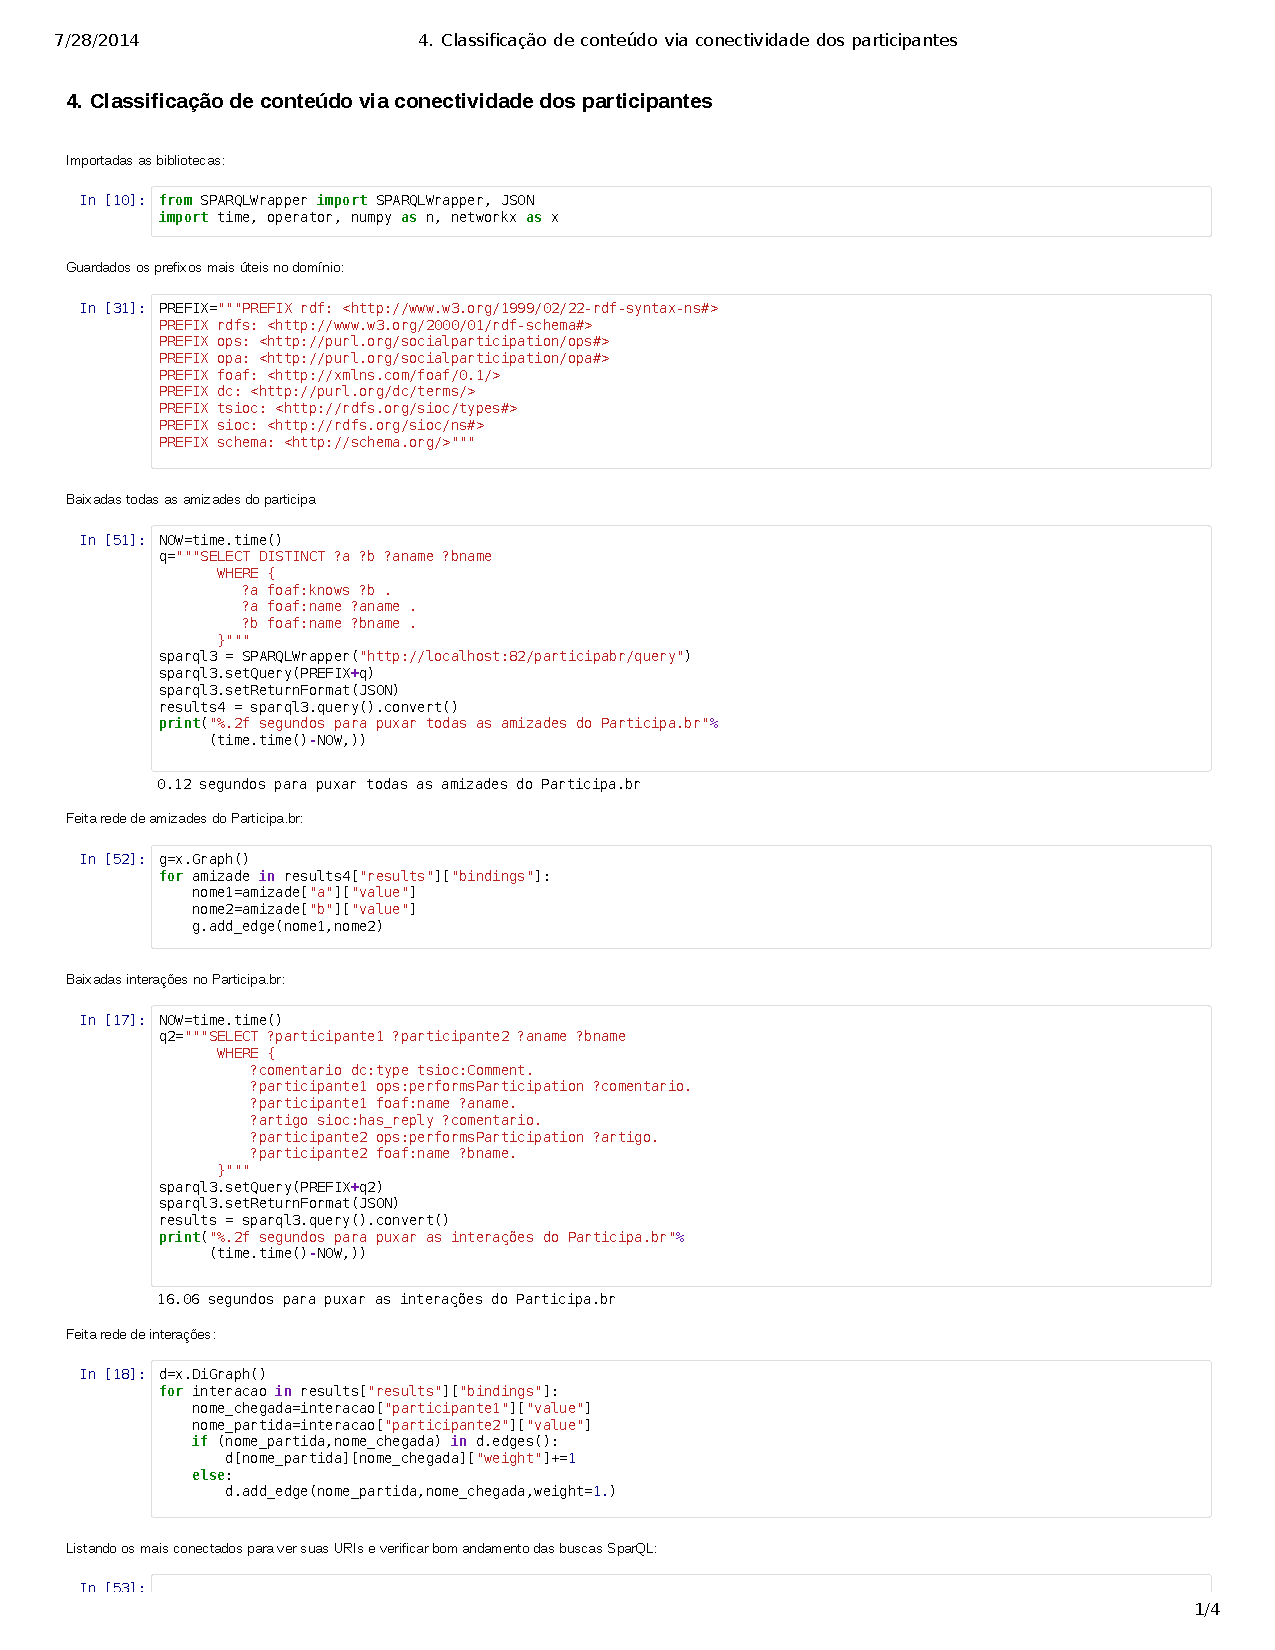
\includepdf[pages=-]{4-ClassificacaoConteudoAutor.pdf}
\invisiblesection{Teste de conexão com o endpoint SparQL que distribui dados do Partipa.br}\label{subsec:csparql}
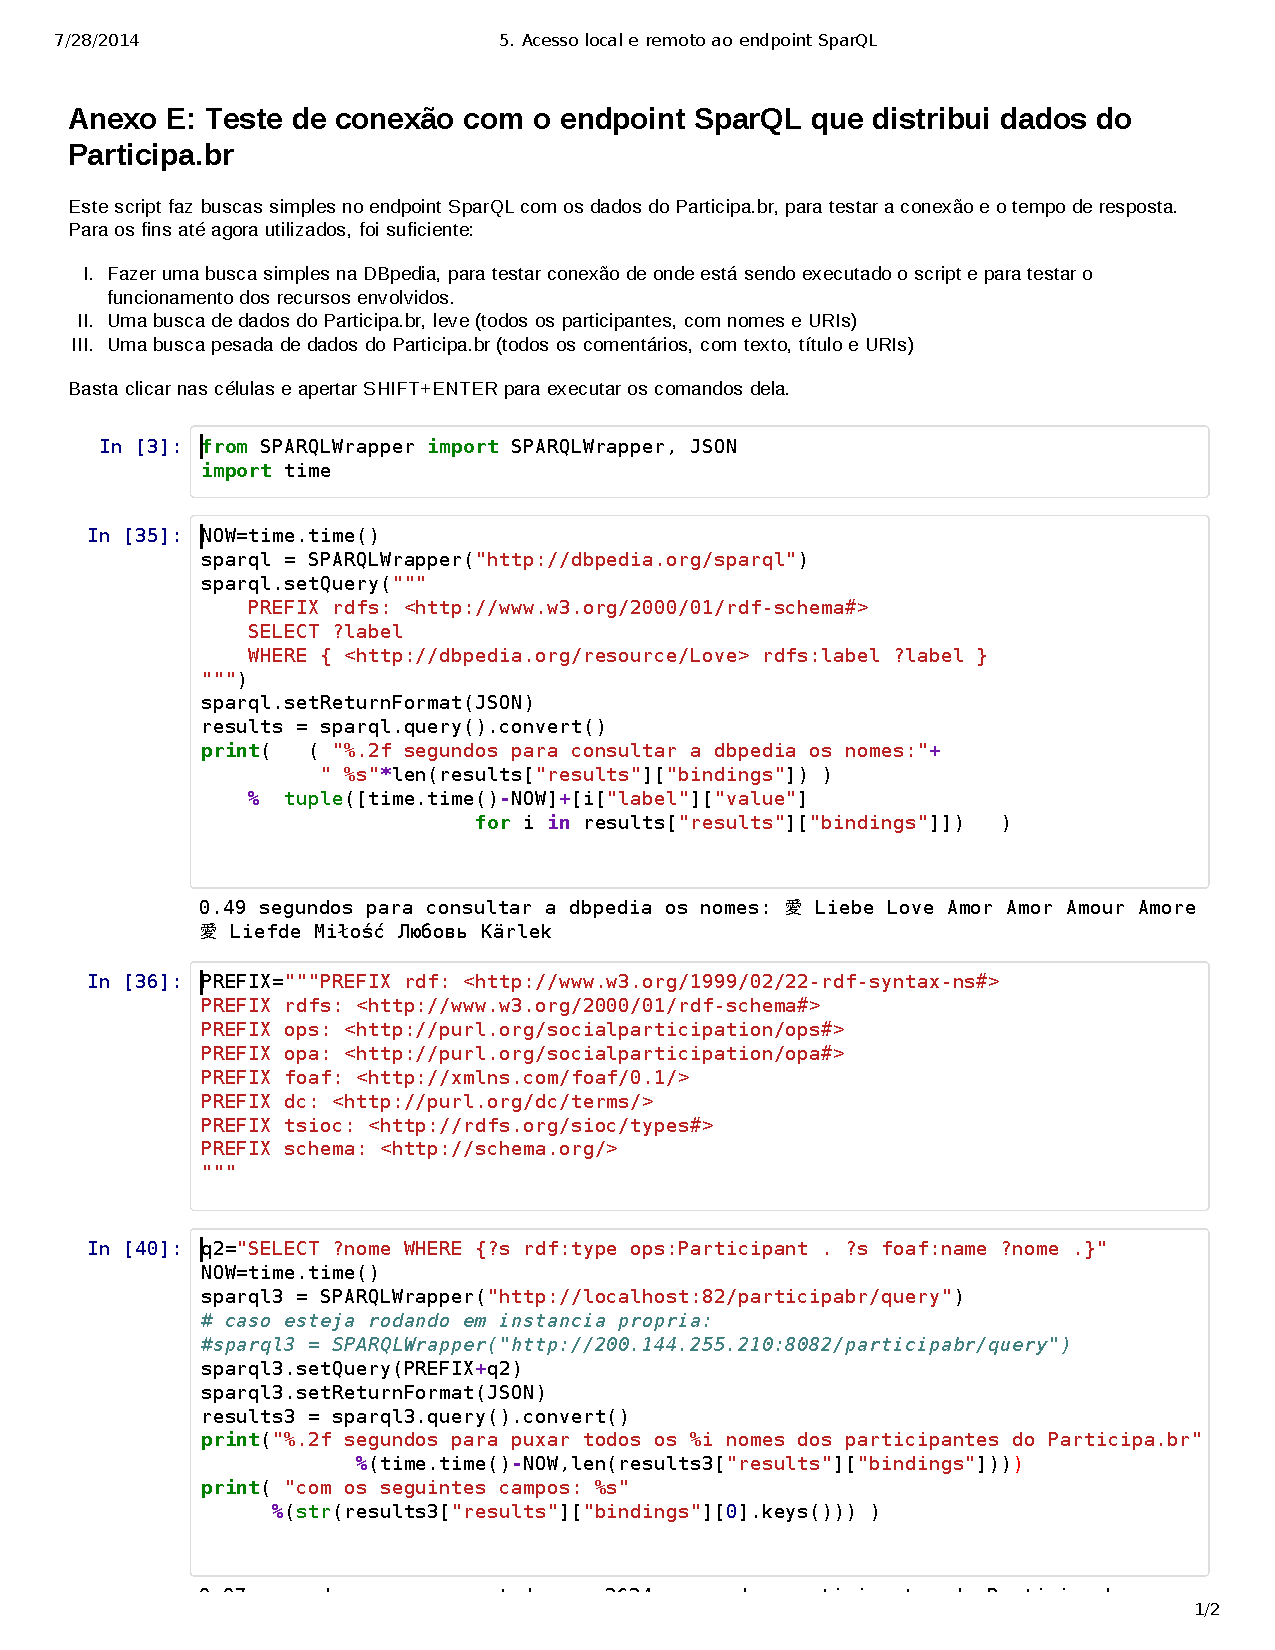
\includepdf[pages=-]{5-SparQLTest.pdf}
\section{Instâncias online}\label{subsec:online}
Alguns recursos desenvolvidos neste trabalho foram disponibilizados online, via http, pela natureza do trabalho e por conveniências. Consistem em ferramentas de streaming, ferramentas de análise, experimentos artísticos e repositórios. Uma seleção pertinente a este escrito é:
\begin{itemize}
    \item IPython Notebook, com os códigos dos Anexos~\ref{subsec:etp}-\ref{subsec:csparql}: \url{http://200.144.255.210:8003}
    \item Endpoint Fuseki/Jena, para acesso aos dados via critérios semânticos: \url{http://200.144.255.210:8082}.
    \item Telões para streaming de estruturas sociais: \url{http://ocupagov.meteor.com}
    \item BrServers, com o resumo ``redes+filtros multidimensionais'': \url{http://gentle-mesa-5082.herokuapp.com/twitter/arenaNETmundial/}
    \item MyNSA, pra coleta de dados do Facebook, Twitter: \url{mynsa.meteor.com}
    \item MMISSA, disposições livres, iniciais e artísticas sobre dados das redes sociais: \url{http://mmissa.meteor.com}
    \item MM, musicalização de estruturas sociais: \url{http://mm.meteor.com}
    \item Respositório de códigos e com este documento: \url{https://github.com/ttm/pnud3}
\end{itemize}
\end{document}
